\documentclass[%
 reprint,
%superscriptaddress,
%groupedaddress,
%unsortedaddress,
%runinaddress,
%frontmatterverbose, 
%preprint,
%preprintnumbers,
%nofootinbib,
%nobibnotes,
%bibnotes,
 amsmath,amssymb,
 aps,
%pra,
%prb,
%rmp,
%prstab,
%prstper,
%floatfix,
]{revtex4-2}

\usepackage{graphicx}  % needed for figures
\usepackage{dcolumn}   % needed for some tables
\usepackage{bm}        % for math
\usepackage{amssymb}   % for math
%\usepackage{hyperref}% add hypertext capabilities
%\usepackage[mathlines]{lineno}% Enable numbering of text and display math
%\linenumbers\relax % Commence numbering lines

%\usepackage[showframe,%Uncomment any one of the following lines to test 
%%scale=0.7, marginratio={1:1, 2:3}, ignoreall,% default settings
%%text={7in,10in},centering,
%%margin=1.5in,
%%total={6.5in,8.75in}, top=1.2in, left=0.9in, includefoot,
%%height=10in,a5paper,hmargin={3cm,0.8in},
%]{geometry}

% Paket float verbessern
\usepackage{scrhack}

% unverzichtbare Mathe-Befehle
\usepackage{amsmath}
% viele Mathe-Symbole
\usepackage{amssymb}
% Erweiterungen für amsmath
\usepackage{mathtools}

% Zahlen und Einheiten
\usepackage[
  locale=US,                   % amerikanische Einstellungen
  separate-uncertainty=true,   % immer Fehler mit \pm
  per-mode=symbol-or-fraction, % / in inline math, fraction in display math
]{siunitx}

% englische Spracheinstellungen
\usepackage[english]{babel}

% schöne Brüche im Text
\usepackage{xfrac}

% Standardplatzierung für Floats einstellen
\usepackage{float}
\floatplacement{figure}{htbp}
\floatplacement{table}{htbp}

% Verbesserungen am Schriftbild
\usepackage{microtype}

\usepackage{natbib}

\begin{document}

\preprint{APS/123-QED}

\title{Measurements of $R(K)$ and $R(K^*)$ with full LHCb Run 1 and 2 data}% Force line breaks with \\
\thanks{Proceeding of LHC Seminar by Renato Quagliani on December 20, 2022}%

\author{Christopher Breitfeld}
\affiliation{Technische Universität Dortmund}%Lines break automatically or can be forced with \\
\email{christopher.breitfeld@tu-dortmund.de}

\date{\today}% It is always \today, today,
             %  but any date may be explicitly specified

\begin{abstract}
    This proceeding presents a novel simultaneous test 
    of muon-electron universality in the decays $B^+\to K^+l^+l^-$ 
    and $B^0\to K^{*0}l^+l^-$. The analysis is performed in two 
    distinct ranges of the invariant dileptonmass $q^2$. The 
    data used in this study is obtained from LHCb Run 1 and 2, with 
    a combined integrated luminosity of $\SI{9}{\per\femto\barn}$. 
    The results demonstrate an improvement over previous measurements 
    and show agreement with the predictions of the Standard Model.
\end{abstract}  

%\keywords{Suggested keywords}%Use showkeys class option if keyword
                              %display desired
\maketitle

The Standard Model of particle physics, a cornerstone in our 
understanding of the fundamental constituents of the universe, 
has been remarkably successful in explaining the behavior and 
interactions of elementary particles. Despite its success, it 
leaves several phenomena unexplained, such as the nature of dark 
matter, the matter-antimatter asymmetry in the universe, and the 
integration of gravity at the quantum level. These gaps in our 
understanding motivate the search for Physics beyond the Standard 
Model (BSM).

One of the key features of the Standard Model is the principle of 
lepton universality (LFU), which posits that all leptons ($e$, $\mu$ and $\tau$) 
should interact in the same way with gauge bosons, apart from differences 
due to their distinct masses. 
Although the leptonflavour in the standard model is not yet theoretically 
understood as a conservation quantity corresponding to a symmetry, 
it has been experimentally confirmed with high precision that W and Z 
bosons couple equally to different leptonflavours \cite{LU_CDF}, \cite{LU_ATLAS}.
Any violation of this principle could be 
a signal of new physics, providing a window into BSM Physics.

In this context, $b\to sl^+l^-$ decays in not resonant regions, provide a 
fertile testing ground, as these decays are sensitive to the Wilson 
coefficients $C_7^{(')}$ corresponding to the electromagnatic dipole operator, 
$C_{9l}^{(')}$ corresponding to the vector operator, and $C_{10,l}^{(')}$ corresponding 
to the axialvector operator. Consequently, LFU measurements can potentially detect 
the influence of hypothetical heavy particles. %Quelle?
The LHCb experiment at CERN, designed to study the 
properties of particles containing b (beauty) and c (charm) quarks, offers 
a unique opportunity to probe these decays with unprecedented precision.
Previous studies of LFU in $b\to sl^+l^-$ decays have indicated a $\num{3.1}\sigma$ 
deviation from the predictions of the Standard Model \cite{previous_RK}, \cite{previous_RK*}. 
Similar deviations have been observed in measurements of angular observables \cite{angular_1}, 
\cite{angular_2}. This proceeding discusses the first simultaneous measurement of electron-muon 
universality in the non-resonant regions of the decays $B^+\to K^+l^+l^-$ and $B^0\to K^{*0}l^+l^-$.

The observable $R$, which is used to test LFU, is defined as
\begin{equation}
    R_{K,K^*}= 
    \frac{\int_{q_a^2}^{q_b^2}\frac{\mathrm{d}\Gamma(B^{(+,0)}\to K^{(+,*0)}\mu^+\mu^-)}{\mathrm{d}q^2}\mathrm{d}q^2}
    {\int_{q_a^2}^{q_b^2}\frac{\mathrm{d}\Gamma(B^{(+,0)}\to K^{(+,*0)}e^+e^-)}{\mathrm{d}q^2}\mathrm{d}q^2} .
    \label{eqn:single_ratio}
\end{equation}

Theoretically, this ratio is predicted to be $\num{1}$, with corrections at 
the percent level \cite{LU_theo}. 
As the decay is depending on the dileptonmass $q^2$, the dataset is divided into four $q^2$ regions:
a non-resonant low $q^2$ region ranging from
$\SIrange{0.1}{1.1}{\giga\electronvolt\squared}$,
a non-resonant central region ranging from
$\SIrange{1.1}{6.0}{\giga\electronvolt\squared}$,
and the regions for the $J/\Psi$ resonance ranging from 
$\SIrange{6.0}{11}{\giga\electronvolt\squared}$
and for the $\Psi(2S)$ resonance ranging from
$\SIrange{11}{15}{\giga\electronvolt\squared}$.

To mitigate uncertainties arising from efficiencies, the double ratio 
\begin{equation}
    R_{K,K^*}= 
    \frac{\frac{N}{\epsilon}(B^{(+,0)}\to K^{(+,*0)}\mu^+\mu^-)}
    {\frac{N}{\epsilon}(B^{(+,0)}\to K^{(+,*0)}e^+e^-)}
    \underbrace{\frac{\frac{N}{\epsilon}(J/\Psi(e^+e^-))}{\frac{N}{\epsilon}(J/\Psi(\mu^+\mu^-))}}_{(r^K_{J/\Psi})^{-1}}
    \label{eqn:double_ratio}
\end{equation}
is defined.

In this equation, $N/\epsilon$ represents the yield of the process, corrected by 
the efficiency. The resonant part, $r^K_{J/\Psi}$, is known to be $\num{1}$ 
\cite{AULCHENKO2014227}. Due to the complexity involved in estimating efficiencies, 
the double ratio provides a more stable measure against systematic uncertainties.

The Large Hadron Collider beauty experiment (LHCb) is one of the four major experiments 
at the Large Hadron Collider (LHC) at CERN. It is designed to conduct high-precision 
measurements of particle decays involving b and c quarks. Given that $b\bar{b}$ pairs 
are boosted in the beam direction, the detector is constructed as a single-arm forward 
spectrometer \cite{LHCb}.

The LHCb trigger system is a three-level system designed to select relevant events from 
the multitude of proton-proton collisions. The first level, known as the Level-0 trigger 
(L0), is hardware-based and reduces the event rate based on information from the calorimeter 
and muon systems. The subsequent levels, HLT1 and HLT2, are software-based. HLT1 applies 
fundamental conditions for partially reconstructed events, while HLT2 utilizes complete 
reconstruction of candidates and employs topological information to further reduce the 
data volume \cite{trigger}.

Particle identification (PID) at LHCb is carried out using information from several 
sub-detectors. The RICH (Ring Imaging Cherenkov) detectors provide PID information by 
measuring the Cherenkov angle of charged particles. The calorimeter system is utilized 
to identify photons, electrons, and hadrons, and to measure their energies. The muon 
system is employed to identify muons. The performance of the PID system is crucial for 
numerous analyses at LHCb, including the measurement of lepton universality in $b\to sll$ 
decays.

The reconstruction of decay in the electron and muon channels presents varying levels of 
complexity, primarily due to three factors. First, electrons emit bremsstrahlung, which adds
a layer of complexity to the reconstruction process. This results in the need for a wider 
fit range, which, while it increases sensitivity to peaking structures, also introduces 
more background into the data. Furthermore, the lineshapes in the data become 
dependent on bremsstrahlung, requiring additional considerations in the data interpretation 
process. Second, the electronic calorimeter's energy resolution is characterized 
by substantial uncertainties. Third, the efficiencies of the L0 triggers for muons and electrons 
differ. These elements collectively contribute to differences in the efficiencies in 
the two channels. 

To neutralize the varying efficiencies of the L0 trigger, one can employ events that are 
triggered independently of the signal, known as Trigger Independent Signal (TIS) events. 
In these instances, the $B$ candidate does not influence the trigger, thereby ensuring that 
the efficiencies between the electron and muon modes are balanced.

The simulations used for the analysis were specifically generated for each data-taking period 
to accurately represent the respective conditions. These simulations take into account a multitude 
of factors that could influence the data, including the specific properties of the detector and 
the environmental conditions during data collection. A crucial aspect of the simulations is the 
modeling of final state radiation, for which the \texttt{PHOTOS} \cite{PHOTOS} program is utilized. 
\texttt{PHOTOS} is a specialized tool developed to accurately simulate the effects of bremsstrahlung in 
final state particle production. By combining these detailed simulations with the data from the 
experiments, the researchers are able to conduct a precise analysis of the decay processes.

To enhance the signal-to-background ratio, two multivariate classifiers are employed. The 
first classifier is designed to distinguish the signal from the combinatorial background, 
which is composed of randomly assembled tracks. This classifier utilizes information about 
the kinematics and geometry of the final state, as well as details about the vertex and the 
quality of the vertex fit.

The second classifier is used to differentiate between the signal and partially reconstructed 
background. These are processes with additional particles $X$ in the final states, such as 
$B\to K l^+l^- X$. If particle $X$ is not correctly reconstructed, the process may be mistakenly 
identified as $B \to K l^+l^-$. This classifier also uses kinematic and geometric features of 
the final states, but additionally, it incorporates information about the spatial and kinematic 
isolation of the final state particles in relation to other reconstructed particles.

To avoid bias, a $k$-folding validation is implemented. Both classifiers are optimized 
simultaneously for each lepton flavor, $q^2$ region, and data-taking period separatly.

% ab hier wirds kompliziert :(

The simulations utilized in the analysis are calibrated to accurately represent the difference 
between electrons and muons. To achieve this, weights are computed via 
$w_i=\epsilon_\text{data}/\epsilon_{Simulation}$ for the $J/\Psi$ resonant decaysin a chain 
for each calibration category $i$. 
The corrections are applied across multiple areas. For instance, the PID is adjusted to ensure 
that the simulation correctly identifies particles as electrons or muons. The tracking of 
particles in the simulation is also corrected to match the real-world data, a process referred 
to as Tracking (TRK) correction.
To accurately represent the kinematics of $B$ particles and the multiplicity of events, adjustments 
are made under the category of $B$ kinematics and event multiplicity (BKIN\&MULT). The simulation's
representation of the hardware trigger's efficiency in real-world data is calibrated under the 
L0 correction.
Similarly, the HLT correction is applied to ensure the simulation accurately represents the software 
trigger. The $B$ decay vertex reconstruction (RECO) correction ensures that the simulation accurately 
represents the reconstruction of the $B$ decay vertex.
Lastly, the $q^2$ resolution and bin-migration (RES) correction is applied to adjust the simulation 
accurately represent the resolution of $q^2$ and the migration of bins. These corrections are crucial 
in ensuring that the simulations provide an accurate representation of the real-world data and thus, 
reliable results.

The effects of these corrections are illustrated in Figure \ref{fig:weights}. 
It is evident that the double ratios $R$ are significantly less influenced by the corrections 
than the single ratio $r^{K^*}_{J/\Psi}$. The single ratio efficiency changes by $\SI{25}{\%}$, 
while all double ratio efficiencies are altered by at most $\SI{5}{\%}$. This demonstrates that 
the double ratio is a more robust observable than the single ratio when it comes to uncertainties 
in the efficiencies.

\begin{figure}
    \centering
    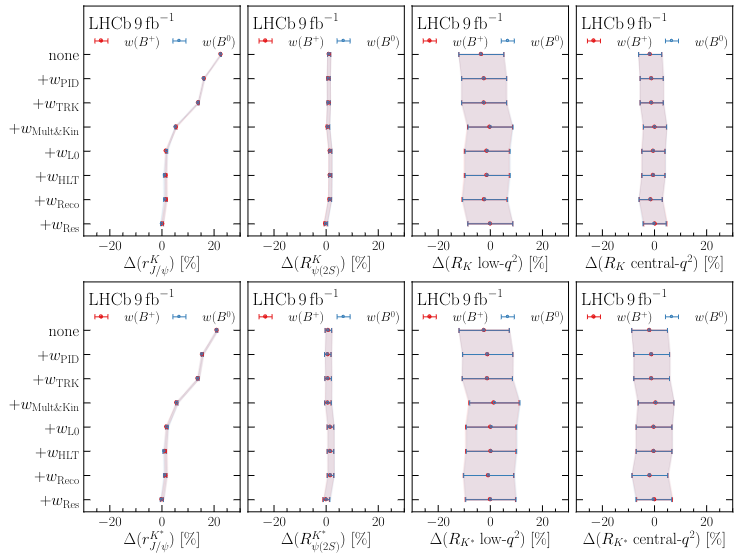
\includegraphics[width=\linewidth]{figures/weights.png}
    \caption{Variation of the efficiencies regarding to the corrections for all four $q^2$ ranges \cite{lhcbcollaboration2022test}.}
    \label{fig:weights}
\end{figure}
To crosscheck all previous steps $r^{K^{(*)}}_{J/\Psi}$ and $R^{K^{(*)}}_{\Psi(2S)}$ are 
calculated. As expected all of them are compatible with $\num{1}$.

The calculation of the doubleratio is performed by a simultaneous maximum-likelihood 
fit to the invariant mass distribution of the reconstructed $B^0$ and $B^+$ in the 
non resonant $q^2$ regions and the $J/\Psi$ resonance. 

In the muon mode, the invariant mass distribution consists only of the signal and 
combinatorial background. 
In the case of the electron, the distribution is much more complicated due to 
residual missidentified hadronic decays and partially reconstructed backgorund. 
Additionally, there are contributions from the resonant $J/\Psi$ decay that extend 
into the central $q^2$ region. 
The signal and these additional components are modeled using various techniques, 
including kernel-density estimators derived from simulated data. 
The combinatorial background is modeled as a decreasing exponential function.
Its distortion by the corrected mass and the selection criteria for partially 
reconstructed events is parametrized by a function derived from background data.
The fit with all determined backgrounds is illustrated in figure \ref{fig:fits}.
The signal yield is then used to calculate the doubleratio using \eqref{eqn:double_ratio}.
\begin{figure}
    \centering
    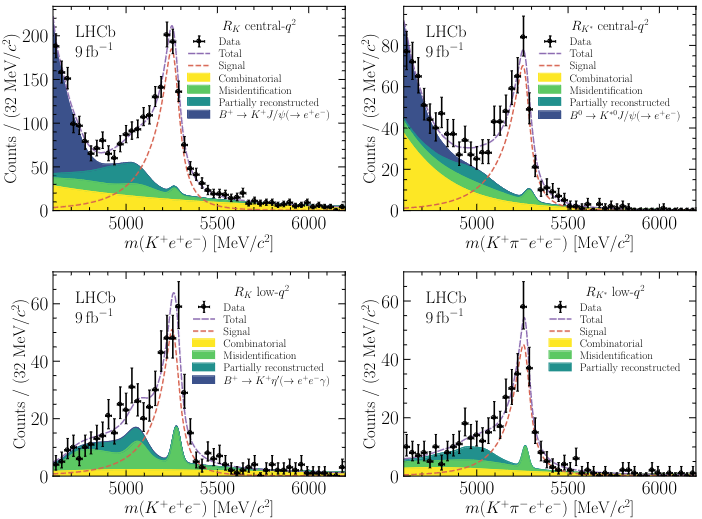
\includegraphics[width=\linewidth]{figures/fits.png}
    \caption{Maximum likelihood fit of the invariant mass distributions in the central $q^2$ (upper) and lower $q^2$ (lower) for the non-resonant decays $B^+\to K^+e^+e^-$ (left) and $B^0\to K^{*0}e^+e^-$ (right) \cite{lhcbcollaboration2022test}.}
    \label{fig:fits}
\end{figure}

The obtained results for the observalbles yield the outcomes
\begin{align*}
    \text{low $q^2$:} 
    &\left\{
    \begin{aligned}
        &R_{K}  \!\!\!\!\!\!\!&&=\, 0.994 \,\substack{+0.090 \\ -0.082}\,\text{(stat)}\,\substack{+0.029 \\ -0.027}\,\text{(syst)}\\
        &R_{K^*}\!\!\!\!\!\!\!&&=\, 0.927 \,\substack{+0.093 \\ -0.087}\,\text{(stat)}\,\substack{+0.036 \\ -0.035}\,\text{(syst)}
    \end{aligned}
    \right. \\
    \text{central $q^2$:} 
    &\left\{
    \begin{aligned}
        &R_{K}  \!\!\!\!\!\!\!&&=\, 0.949 \,\substack{+0.042 \\ -0.041}\,\text{(stat)}\,\substack{+0.022 \\ -0.022}\,\text{(syst)}\\
        &R_{K^*}\!\!\!\!\!\!\!&&=\, 1.027 \,\substack{+0.072 \\ -0.068}\,\text{(stat)}\,\substack{+0.027 \\ -0.026}\,\text{(syst)}.
    \end{aligned}
    \right.
\end{align*}

The dominant sources of systematic uncertainty in the modeling of 
invariant mass distributions arise from the data-driven modeling 
of misidentified backgrounds. These uncertainties vary from 
$\SI{2.0}{\%}$ to $\SI{2.5}{\%}$, depending on the specific observable. 
Another significant source of uncertainty is associated with the 
stability of the single ratios $r^{K^{(*)}}_{J/\Psi}$, which depends on 
the kinematics and geometry of the decay. However, excluding the low 
$q^2$ region for $R_{K^*}$, this uncertainty contributes significantly 
less than the uncertainty stemming from the modeling of misidentified 
backgrounds. Overall, the statistical uncertainties dominate the total 
uncertainty of the results.
The measurements of $R_K$ and $R_K^*$ in the low $q^2$ 
and central $q^2$ regions currently represent the most 
precise tests of Lepton Flavour Universality (LFU). 
Contrary to previous measurements, this analysis aligns 
with the Standard Model predictions, with an agreement of 
$\num{0.2}\sigma$, as shwon in figure \ref{fig:results}. 
This study underscores the importance of understanding 
electron misidentification and also demonstrates the 
benefits of a double-ratio approach in minimizing 
systematic uncertainties. The statistical uncertainties 
significantly outweigh the systematic ones in this 
analysis, suggesting that a larger dataset is required 
to improve the precision of the measurement.

\begin{figure}
    \centering
    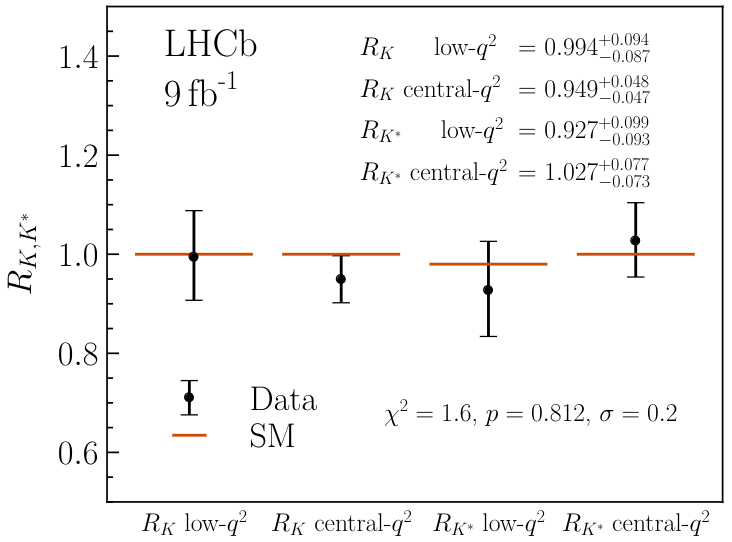
\includegraphics[width=\linewidth]{figures/results.png}
    \caption{Graphical comparison of the measured results of $R_K$ and $R_{K^*}$ in the low and central $q^2$ range with the standard model predictions \cite{lhcbcollaboration2022measurement}.}
    \label{fig:results}
\end{figure}

While the LFU tensions with respect to the Standard Model 
appear to be of systematic origin, the tensions related to 
the branching fractions $\mathcal{B}(B^{(0,+)}\to K^{(+,*0)}l^+l^-)$ 
remain \cite{Branchingfraction}.

The upcoming LHCb Run 3, with its increased statistics and 
new detector enhancements, including the trigger system, is 
expected to further refine the precision of LFU tests.
%\input{content/entwurf.tex}

\bibliography{lit} % Ersetzen Sie "references" durch den Namen Ihrer .bib-Datei

\end{document}